
\section{GRPO for Memory Evolution}
\label{app:grpo}

For completeness, we summarize the GRPO objective for the multi-turn memory evolution process. Following MemAgent~\citep{yu2025memagent}, we optimize memory evolution over groups of trajectories. For a given input \((\mathcal{H}, x)\), the current policy \( \pi_\phi \) generates a group of \(G\) trajectories \(\{\tau_i\}_{i=1}^G\), with corresponding rewards \(\{R_i\}_{i=1}^G\). In the multi-conversation setting, each trajectory \(\tau_i\) is further decomposed into \(n_i\) conversations,
\[
\tau_i = \{\tau_{i,1}, \tau_{i,2}, \dots, \tau_{i,n_i}\},
\]
where \(\tau_{i,j}\) denotes the token sequence of the \(j\)-th conversation. GRPO normalizes rewards within each group and defines a group-relative advantage:
\begin{equation}
\widehat{A}_i
=
\frac{R_i - \mathrm{mean}(\{R_j\}_{j=1}^G)}{\mathrm{std}(\{R_j\}_{j=1}^G)}.
\end{equation}
This advantage is then assigned to all token-level actions in \(\tau_i\), including both memory-update tokens and answer tokens across all conversations. Let \(r_{i,j,t}(\phi)\) denote the importance-sampling ratio between the current policy and a frozen reference policy \(\pi_{\text{ref}}\) at token step \(t\) in the \(j\)-th conversation of trajectory \(\tau_i\). The multi-conversation GRPO objective is written as
\begin{equation}
\begin{aligned}
&J_{\mathrm{GRPO}}(\phi)
=
\mathbb{E}\Bigg[
\frac{1}{G}
\sum_{i=1}^G
\frac{1}{\sum_{j=1}^{n_i} |\tau_{i,j}|}
\sum_{j=1}^{n_i}
\sum_{t \in \tau_{i,j}}
\\[-2mm]
&\min\!\Big(
r_{i,j,t}(\phi)\widehat{A}_i,
\mathrm{clip}\!\big(r_{i,j,t}(\phi),1-\epsilon,1+\epsilon\big)\widehat{A}_i
\Big)
\\
&\qquad
-\beta\,\mathrm{KL}\!\left(\pi_\phi\,\|\,\pi_{\text{ref}}\right)
\Bigg].
\end{aligned}
\end{equation}

\section{Hyperparameter Settings} \label{app:hyperparameter}

We summarize the hyperparameter settings for training and inference in Table~\ref{tab:hyperparameters}.

\begin{table}[t]
\centering
\small
\setlength{\tabcolsep}{4pt}
\renewcommand{\arraystretch}{1.05}
\begin{tabular}{l l}
\toprule
\textbf{Phase} & \textbf{Hyperparameters} \\
\midrule
\textbf{Training (Stage 1)} & Context = RAG \\
& Round size = 512 \\
& Optimization steps = $\{10, 30, 50, 70\}$ \\
& Temperature = 1.0 \\
& Top-$p$ = 1.0 \\
& Max output tokens = 2048 \\
\midrule
\textbf{Training (Stage 2)} & Context = RAG \\
& Batch size = 4 \\
& Round size = 512 \\
& Learning rate = $1 \times 10^{-6}$ \\
& Temperature = 1.0 \\
& Top-$p$ = 1.0 \\
& Rollout batch size = 8 \\
& Rollout $n$ = \{2,4,8\} \\
& Epochs = 5 \\
& Max output tokens = 2048 \\
\midrule
\textbf{Inference} & Context = Full history \\
& Round size = $\{1\textsc{k}, 2\textsc{k}, 4\textsc{k}, 8\textsc{k}, 16\textsc{k}\}$ \\
& Serving = vLLM \\
& Max output tokens = 2048 \\
& Temperature = 0.0 \\
\bottomrule
\end{tabular}
\caption{Hyperparameter settings used for training and inference.}
\label{tab:hyperparameters}
\end{table}




\section{Datasets} 
\label{app:Datasets}


\subsection{PersonaMem Dataset}
\label{app:personamem-dataset}

PersonaMem \cite{personamem} is a large-scale benchmark for evaluating long-term personalization in conversational LLMs. It contains interaction histories for \textbf{20 simulated personas}, each designed with rich static attributes (e.g., demographics and occupation) and dynamic traits and preferences that evolve over time across \textbf{15 diverse real-world task domains} such as food recommendation, travel planning, and therapy consultation. For every persona, multi-session conversations are constructed in which the user engages with a chatbot over \textbf{7 types of in-situ queries} that probe different personalization capabilities (e.g., recalling user facts, tracking preference evolution, and providing preference-aligned suggestions). Each session consists of 15-30 user–assistant turns, and histories are instantiated at three context scales by concatenating 10, 20, or 60 sessions, yielding approximate context lengths of 32k, 128k, and 1M tokens, respectively. At evaluation time, models must select appropriate responses to user queries conditioned on the interaction history, thereby testing their ability to evolve over dynamic user profiles. The main statistics of PersonaMem are summarized in Table~\ref{tab:personamem-stats}.

\begin{table}[t]
\setlength{\tabcolsep}{4pt}
  \centering
  \begin{tabular}{lccc}
    \toprule
    \textbf{Statistic} & \multicolumn{3}{c}{\textbf{PersonaMem}} \\
    \midrule
    Tokens per history        & \textasciitilde 32k   & \textasciitilde 128k  & \textasciitilde 1M     \\
    \# QA pairs               & 589   & 2727  & 2674   \\
    \# Sessions per history   & 10    & 20    & 60     \\
    Avg.\ \# utterances       & 167.1 & 758.3 & 3607.9 \\
    \bottomrule
  \end{tabular}
  \caption{Statistics of the PersonaMem dataset at different context lengths. Token counts denote the approximate total context length per interaction history; utterance counts are averaged over histories.}
  \label{tab:personamem-stats}
\end{table}

\begin{table}[t]
\centering
% \setlength{\tabcolsep}{6pt}
\begin{tabular}{l r}
\toprule
\textbf{Statistic} & \textbf{Value} \\
\midrule
Explicit queries & 1{,}000 \\
Implicit queries & 1{,}000 \\
Maximum inserted conversations & 24 \\
Maximum inserted turns & 326 \\
Avg.\ turns / conversation & 13.58 \\
Total tokens & 108{,}102 \\
Avg.\ tokens / conversation & 4{,}504.25 \\
\bottomrule
\end{tabular}
\caption{Dataset statistics for PrefEval multiple-choice classification.}
\label{tab:prefeval_stats}
\end{table}

\begin{table}[t]
\centering
\small
\begin{tabular}{lrrrrr}
\toprule
\textbf{User} & \textbf{Queries} & \textbf{Corpus} & \textbf{Conv.} & \textbf{AI} & \textbf{E-com.} \\
\midrule
1 & 48 & 110 & 84 & 23 & 3 \\
2 & 43 & 90  & 78 & 8  & 4 \\
3 & 42 & 64  & 51 & 12 & 1 \\
4 & 46 & 85  & 71 & 14 & 0 \\
5 & 44 & 84  & 59 & 21 & 4 \\
6 & 40 & 94  & 79 & 14 & 1 \\
\midrule
\textbf{Sum} & 263 & 527 & 422 & 92 & 13 \\
\bottomrule
\end{tabular}
\caption{Statistics of the PersonaBench subset across six users. \textit{Corpus} is the sum of \textit{Conv.}, \textit{AI}, and \textit{E-com.}.}
\label{tab:personabench-stats}
\end{table}


\subsection{PrefEval Dataset}
PrefEval is a long-context, multi-session benchmark for evaluating whether LLMs can infer, retrieve, and act on user preferences in realistic conversational settings, with an emphasis on four aspects: preference inference, long-context retrieval, preference following, and personalization proactiveness. The dataset comprises 1{,}000 unique preference--query pairs, and spans 20 everyday topics grouped into seven domains: \textit{Entertainment} (Shows, Music \& Books, Sports, Games), \textit{Travel} (Activities, Restaurant, Hotel, Transport), \textit{Lifestyle} (Dietary, Beauty, Fitness, Health), \textit{Shopping} (Home, Fashion, Motors, Technology), \textit{Education} (Resources, Learn Styles), \textit{Professional Ownership}, and \textit{Professional Work Style}. PrefEval supports two evaluation formats: a free-form generation setting and a 4-way multiple-choice classification setting in which exactly one option is consistent with the stated preference. To stress long-range personalization, the benchmark inserts unrelated multi-session dialogue turns between the preference revelation and the final query. In our experiments, we use 1{,}000 explicit and 1{,}000 implicit instances under the multiple-choice classification setting, and insert 50 intervening turns as distractor context; summary statistics of our subset are reported in Table~\ref{tab:prefeval_stats}.


\subsection{PersonaBench Dataset}

PersonaBench \cite{tan2025personabench} is a benchmark designed to evaluate personalized retrieval and question answering grounded in user-specific context. For each user, it provides a heterogeneous personal corpus comprising (i) conversations with friends (\textit{Conv.}), (ii) dialogues with AI assistants (\textit{AI}), and (iii) e-commerce purchase histories (\textit{E-com.}). The evaluation queries are typically short and underspecified, requiring models to resolve implicit intent by grounding responses in evidence distributed across the user’s historical interactions and behaviors. This setting tests a model’s ability to align with diverse, user-dependent semantics under realistic contextual ambiguity. Table~\ref{tab:personabench-stats} summarizes the per-user query counts and corpus statistics for the six-user subset used in our experiments.


\section{Comparison in Different Categories} \label{app:ComparisoninDifferentCategories}

\paragraph{Comparison in Different Categories of PersonaMem.}

\begin{table*}[ht]
\centering
\small
\setlength{\tabcolsep}{3pt}
% \renewcommand{\arraystretch}{0.9}
\begin{tabular}{p{2.2cm}|M{1.4cm}M{1.4cm}M{1.4cm}M{1.4cm}M{1.4cm}M{1.4cm}M{1.4cm}|M{1.4cm}}
\toprule
\textbf{Method}  &
\textbf{Recall facts} &
\textbf{Suggest ideas} &
\textbf{Latest prefs} &
\textbf{Prefs evolve} &
\textbf{Update reasons} &
\textbf{Aligned recs} &
\textbf{New Scenarios} &
\textbf{Overall} \\
\midrule
\multicolumn{9}{c}{\cellcolor{cvprblue!12}\textit{\textbf{$\blacktriangledown$ 32K memory corpus data}}} \\
\midrule
Long Context & 28.93 & 11.39 & - & 44.07 & 61.25 & 35.56 & 15.22 & 34.36 \\
RAG          & 42.98 & 15.19 & - & 59.32 & 80.00 & 51.11 & 36.96 & 48.67 \\
Mem0         & 47.93 & \textbf{19.41} & - & 46.61 & 79.58 & 57.04 & 42.75 & 48.53 \\
A-Mem        & 47.11 & 10.13 & - & 61.86 & 80.00 & 44.44 & 30.43 & 48.26 \\
LightMem     & 52.07 & 10.13 & - & 65.25 & 77.50 & 51.11 & 32.61 & 50.72 \\
MemAgent     & 54.55 &  8.86 & - & 65.25 & 76.25 & 57.78 & 54.35 & 53.58 \\
Mem-$\alpha$ & 57.02 &  7.59 & - & 64.41 & 72.50 & 60.00 & 54.35 & 53.37 \\
 \ourmodel(Ours) & \textbf{59.50} &  8.86 & - & \textbf{68.64} & \textbf{81.25} & \textbf{62.22} & \textbf{56.52} & \textbf{57.06} \\
\midrule
\multicolumn{9}{c}{\cellcolor{blue!10}\textit{\textbf{$\blacktriangledown$ 128K memory corpus data}}} \\
\midrule
Long Context & 18.12 & 23.36 & 20.62 & 38.62 & 39.77 & 21.70 & 16.99 & 25.05 \\
RAG          & \textbf{54.37} & \textbf{19.67} & 36.45 & 52.69 & 58.71 & 41.94 & 29.61 & 38.90 \\
Mem0         & 56.25 & 20.49 & 37.77 & 55.09 & 57.20 & 41.64 & 29.13 & 39.67 \\
A-Mem        & 36.88 & 16.19 & 38.73 & 59.88 & 62.50 & 35.19 & 28.16 & 38.22 \\
LightMem     & 40.00 & 17.42 & 42.33 & 61.08 & \textbf{64.02} & 35.48 & 25.73 & 39.93 \\
MemAgent     & 50.62 & 10.86 & 49.40 & 61.68 & 59.47 & 47.80 & 35.44 & 43.59 \\
Mem-$\alpha$ & 48.75 & 10.45 & 50.12 & 59.28 & 54.55 & 47.21 & 36.89 & 42.86 \\
 \ourmodel(Ours) & 52.50 & 11.68 & \textbf{54.44} & \textbf{66.47} & \textbf{64.02} & \textbf{51.61} & \textbf{38.35} & \textbf{47.24} \\
\bottomrule
\end{tabular}
\caption{Category-wise accuracy (\%) on PersonaMem under 32K and 128K interaction histories. “--” indicates the category is not available in the dataset.}
\label{tab:personamem_comparison}
\end{table*}


\begin{table*}[!htbp]
\centering
\small
\setlength{\tabcolsep}{3pt}
% \renewcommand{\arraystretch}{0.9}
\begin{tabular}{p{2.2cm}|M{1.4cm}M{1.4cm}M{1.4cm}M{1.4cm}M{1.4cm}M{1.4cm}M{1.4cm}|M{1.4cm}}
\toprule
\textbf{Method}  &
\textbf{Travel} &
\textbf{Entertain} &
\textbf{Lifestyle} &
\textbf{Shop} &
\textbf{Education} &
\textbf{Professional} &
\textbf{Pet} &
\textbf{Overall} \\
\midrule
\multicolumn{9}{c}{\cellcolor{cvprblue!12}\textit{\textbf{$\blacktriangledown$ Explicit Memory}}} \\
\midrule
Long Context & 31.78 & 30.77 & 32.70 & 30.00 & 32.94 & 27.78 & 39.53 & 31.70 \\
RAG         & 45.33 & 52.04 & 47.87 & 45.79 & 42.35 & 58.33 & 48.84 & 47.80 \\
Mem0        & 58.41 & 61.99 & 57.35 & 53.68 & 54.12 & 69.44 & 46.51 & 57.60 \\
A-Mem       & 62.15 & 69.23 & 60.19 & 61.05 & 54.12 & 66.67 & 55.81 & 62.30 \\
LightMem    & 65.42 & 68.33 & 65.40 & 62.11 & 56.47 & 66.67 & 53.49 & 64.20 \\
MemAgent    & 71.03 & \textbf{77.83} & 70.62 & 71.05 & 62.35 & \textbf{83.33} & \textbf{74.42} & 72.30 \\
Mem-$\alpha$& 78.50 & 73.76 & 67.30 & 70.00 & 65.88 & 77.78 & 67.44 & 71.90 \\
\ourmodel(Ours) & \textbf{82.24} & 76.92 & \textbf{84.83} & \textbf{82.11} & \textbf{85.88} & \textbf{83.33} & 67.44 & \textbf{81.30} \\
\midrule
\multicolumn{9}{c}{\cellcolor{blue!10}\textit{\textbf{$\blacktriangledown$ Implicit Memory}}} \\
\midrule
Long Context & 30.84 & 27.60 & 34.12 & 29.47 & 34.12 & 25.00 & 34.88 & 30.80 \\
RAG         & 26.17 & 41.18 & 33.65 & 29.47 & 30.59 & 13.89 & 44.19 & 32.40 \\
Mem0        & 43.93 & 51.13 & 48.34 & 42.11 & 44.71 & 30.56 & 60.47 & 46.40 \\
A-Mem       & 51.40 & 55.20 & 55.45 & 47.37 & 54.12 & 50.00 & 58.14 & 52.80 \\
LightMem    & 50.47 & 60.63 & 58.77 & 51.58 & 47.06 & 44.44 & 65.12 & 54.80 \\
MemAgent    & 59.35 & 66.52 & 65.88 & 63.68 & 56.47 & 52.78 & \textbf{81.40} & 63.60 \\
Mem-$\alpha$& 61.68 & 66.52 & 62.09 & 61.05 & 60.00 & 52.78 & 67.44 & 62.50 \\
 \ourmodel(Ours) & \textbf{64.02} & \textbf{69.23} & \textbf{73.93} & \textbf{72.63} & \textbf{70.59} & \textbf{63.89} & 74.42 & \textbf{69.90} \\
\bottomrule
\end{tabular}
\caption{Domain-wise accuracy (\%) on PrefEval multiple-choice classification under Explicit vs.\ Implicit preference.}
\label{tab:prefeval_category}
\end{table*}


\begin{table*}[!htbp]
\centering
\small
% \setlength{\tabcolsep}{3pt}
% \renewcommand{\arraystretch}{0.95}
\begin{tabular}{l|c c c c c|c c c c c}
\toprule
\textbf{Method} &
\makecell{\textbf{Basic}\\\textbf{Info}} &
\makecell{\textbf{Pref.}\\\textbf{(Easy)}} &
\makecell{\textbf{Pref.}\\\textbf{(Hard)}} &
\textbf{Social} &
\textbf{Overall} &
\makecell{\textbf{Basic}\\\textbf{Info}} &
\makecell{\textbf{Pref.}\\\textbf{(Easy)}} &
\makecell{\textbf{Pref.}\\\textbf{(Hard)}} &
\textbf{Social} &
\textbf{Overall} \\
\midrule
\multicolumn{1}{c|}{} &
\multicolumn{5}{c|}{\cellcolor{cvprblue!12}\textit{\textbf{$\blacktriangledown$ Without Noise Memory}}} &
\multicolumn{5}{c}{\cellcolor{blue!10}\textit{\textbf{$\blacktriangledown$ With 0.3 Noise Memory}}} \\
\midrule
Long Context  & \textbf{29.23} & 34.41 & 24.51 & 29.36 & 29.00 & 21.15 & 22.24 & 18.78 & 13.55 & 19.10 \\
RAG           & 24.32 & 34.06 & 32.77 & 33.68 & 29.09 & 26.14 & 39.29 & 28.63 & 26.53 & 28.16 \\
Mem0          & 19.23 & 19.09 & 18.80 & 12.58 & 17.60 & 17.41 & 29.08 & 21.87 & 18.39 & 19.75 \\
A-Mem         & 25.69 & 34.04 & 34.46 & 34.90 & 30.32 & 27.00 & \textbf{39.65} & 26.94 & \textbf{27.61} & 28.56 \\
LightMem      & 18.92 & 20.41 & 21.40 & 16.96 & 19.08 & 21.25 & 22.60 & 18.52 & 11.82 & 18.74 \\
MemAgent      & 14.32 & 31.09 & 26.58 & 21.48 & 20.05 & 16.30 & 32.36 & 18.76 & 19.77 & 19.36 \\
Mem-$\alpha$  & 14.91 & 25.92 & 30.03 & 19.55 & 19.92 & 11.87 & 27.71 & 26.00 & 15.52 & 17.02 \\
\ourmodel     & 26.74 & \textbf{34.61} & \textbf{37.02} & \textbf{38.95} & \textbf{32.27} & \textbf{29.81} & 35.12 & \textbf{29.92} & 27.48 & \textbf{29.89} \\
\midrule
\multicolumn{1}{c|}{} &
\multicolumn{5}{c|}{\cellcolor{cvprblue!12}\textit{\textbf{$\blacktriangledown$ With 0.5 Noise Memory}}} &
\multicolumn{5}{c}{\cellcolor{blue!10}\textit{\textbf{$\blacktriangledown$ With 0.7 Noise Memory}}} \\
\midrule
Long Context  & 18.65 & 16.52 & 17.90 & 16.70 & 17.83 & 11.25 & 22.26 & 18.62 & 7.75  & 13.00 \\
RAG           & 22.45 & 27.49 & 22.58 & 27.95 & 24.31 & 18.38 & 31.83 & 25.85 & 26.05 & 23.00 \\
Mem0          & 18.33 & 24.31 & 23.79 & 15.04 & 19.22 & 15.07 & 21.38 & 21.58 & 18.76 & 17.80 \\
A-Mem         & 22.28 & 23.64 & \textbf{28.12} & \textbf{29.73} & 25.19 & 18.42 & 29.96 & \textbf{28.11} & 31.42 & 24.45 \\
LightMem      & 22.85 & 20.47 & 17.09 & 14.59 & 19.65 & 20.30 & 19.80 & 17.35 & 12.00 & 17.80 \\
MemAgent      & 13.40 & 16.73 & 21.13 & 19.27 & 16.51 & 13.76 & 26.45 & 23.01 & 18.44 & 17.92 \\
Mem-$\alpha$  & 11.20 & 17.31 & 22.36 & 22.28 & 16.43 & 12.42 & 22.66 & 18.55 & 16.42 & 15.59 \\
\ourmodel     & \textbf{23.82} & \textbf{33.01} & 23.19 & 29.21 & \textbf{25.99}& \textbf{20.62} & \textbf{36.91} & 27.09 & \textbf{27.00} & \textbf{25.09} \\
\bottomrule
\end{tabular}
\caption{Category-wise macro F1 (\%) on PersonaBench for the six-user subset under different noise rates injected into the memory bank.}
\label{tab:personabench_category}
\end{table*}


Table~\ref{tab:personamem_comparison} reports category-wise results on PersonaMem under 32K and 128K interaction histories. Across both scales, \ourmodel achieves the best overall performance (57.06 at 32K; 47.24 at 128K), and the gains are concentrated on memory-dependent personalization abilities. On 32K histories, \ourmodel leads in  Recall facts (59.50), Prefs evolve (68.64), Update reasons (81.25), Aligned recs (62.22), and New Scenarios (56.52), which jointly drives a clear margin over the strongest baselines (e.g., 57.06 vs.\ 53.58 for MemAgent). When scaling to 128K, \textit{Long Context} degrades sharply overall (25.05), while memory-based methods remain substantially stronger; within them, \ourmodel stays best-performing and ranks first on Latest prefs (54.44), Prefs evolve (66.47), Aligned recs (51.61), and New Scenarios (38.35). In contrast, Suggest ideas is not a strength for \ourmodel (8.86/11.68), where methods that do not emphasize memory evolution (e.g., Mem0 or Long Context) are higher, indicating that our improvements primarily come from better tracking and applying evolving persona preferences rather than open-ended QA. Overall, the category-wise gains suggest that explicitly \emph{structuring} memory operations and then \emph{selecting} what to keep is most effective for preference-heavy queries, and the advantage becomes more pronounced as the interaction history grows longer.


\paragraph{Comparison in Different Categories of PrefEval.}


Table~\ref{tab:prefeval_category} breaks down PrefEval performance by domain under \textbf{Explicit} and \textbf{Implicit} preference settings. Under Explicit Memory, \ourmodel attains the best overall accuracy (81.30) and shows consistently strong gains on preference-heavy domains, ranking first on Travel (82.24), Lifestyle (84.83), Shop (82.11), and Education (85.88), while remaining competitive on \textbf{Entertain} (76.92) and Professional (83.33). A notable exception is Pet, where \ourmodel (67.44) trails MemAgent (74.42), suggesting that not all topics benefit equally from the same memory update behavior. Under Implicit Memory, the task becomes more challenging for all methods, yet \ourmodel again leads overall (69.90) and improves most clearly on domains that require inferring latent preferences from context, including Lifestyle (73.93), Shop (72.63), Education (70.59), and Professional (63.89). Compared with memory-bank baselines (Mem0/A-Mem/LightMem), the advantage of \ourmodel is broad across domains in both settings, indicating that it better resists long-range distractors and preserves preference-relevant signals. Overall, these domain-wise results reflect PrefEval’s construction: the inserted unrelated turns make long-range preference retrieval and faithful preference following the main bottlenecks, and \ourmodel improves most on domains where precise preference identification and consistent application are essential.



\paragraph{Comparison in Different Categories of PersonaBench.}

Table~\ref{tab:personabench_category} reports category-wise macro F1 on PersonaBench under increasing noise in the memory bank, where queries are short and underspecified, and evidence is distributed across heterogeneous user corpora (Table~\ref{tab:personabench-stats}). Without noise, \ourmodel achieves the best overall score (32.27) and is particularly strong on preference- and interaction-driven categories, leading on Pref.\ (Hard) (37.02) and Social (38.95), while remaining competitive on Pref.\ (Easy) (34.61); in contrast, Basic Info favors direct long-context inclusion (Long Context: 29.23 vs.\ \ourmodel: 26.74), suggesting that simple factual lookup is less dependent on selective memory evolution. As noise increases, all methods degrade, but \ourmodel remains the best overall method at every noise level (29.89 at 0.3; 25.99 at 0.5; 25.09 at 0.7), indicating stronger robustness to irrelevant or misleading memory entries. The category breakdown further shows that \ourmodel maintains clear advantages on Pref.\ (Easy) under heavier noise (36.91 at 0.7), while the performance gap on Pref.\ (Hard) and Social narrows against strong baselines (e.g., A-Mem), reflecting that fine-grained preference grounding and social inference are the most sensitive to noisy evidence. Overall, the results highlight that \ourmodel is most beneficial when personalization requires resolving implicit intent over long, heterogeneous histories, and it degrades more gracefully as the memory bank becomes noisier.


\section{Additional Experiments}

\subsection{Comparison with Post-Training Baselines}
\begin{table*}[ht]
\centering
\small
\setlength{\tabcolsep}{3pt}
\begin{tabular}{p{2.2cm}|M{1.4cm}M{1.4cm}M{1.4cm}M{1.4cm}M{1.4cm}M{1.4cm}M{1.4cm}|M{1.4cm}}
\toprule
\textbf{Method}  &
\textbf{Recall facts} &
\textbf{Suggest ideas} &
\textbf{Latest prefs} &
\textbf{Prefs evolve} &
\textbf{Update reasons} &
\textbf{Aligned recs} &
\textbf{New Scenarios} &
\textbf{Overall} \\
\midrule
Frozen & 28.93 & 11.39 & - & 44.07 & 61.25 & 35.56 & 15.22 & 34.36 \\
SFT    & 42.15 & \textbf{15.19} & - & 55.93 & \textbf{81.25} & 48.89 & 28.26 & 46.83 \\
PPO    & 51.24 & \textbf{15.19} & - & 60.17 & 75.00 & 44.44 & 36.96 & 49.49 \\
GRPO   & 52.07 & 16.46 & - & 63.56 & 71.25 & 46.67 & 36.96 & 50.31 \\
\midrule
\ourmodel & \textbf{59.50} & 8.86 & - & \textbf{68.64} & \textbf{81.25} & \textbf{62.22} & \textbf{56.52} & \textbf{57.06} \\
\bottomrule
\end{tabular}
\caption{Comparison with different post-training methods on PersonaMem 32K memory corpus data.}
\label{tab:posttrain_comparison_32k}
\end{table*}




Table~\ref{tab:posttrain_comparison_32k} compares \ourmodel with standard post-training baselines trained on the same 300 PersonaMem training data, where the baselines do not perform memory evolution and instead optimize question answering directly. Moving from Frozen to SFT and then to PPO/GRPO yields steady overall improvements (34.36$\rightarrow$46.83$\rightarrow$49.49/50.31), indicating that post-training helps, but the gains are uneven across personalization skills. In contrast, \ourmodel achieves the best overall score (57.06) and leads on most categories, including Recall facts (59.50), Prefs evolve (68.64), Aligned recs (62.22), and New Scenarios (56.52). This pattern is consistent with our design: by explicitly internalizing memory extraction, update, and forgetting into a dedicated memory-evolution mechanism, \ourmodel improves long-horizon preference tracking and generalization beyond what QA-only post-training captures.





\subsection{Evaluation of Preference Retention}

\begin{figure*}[t]
\centering
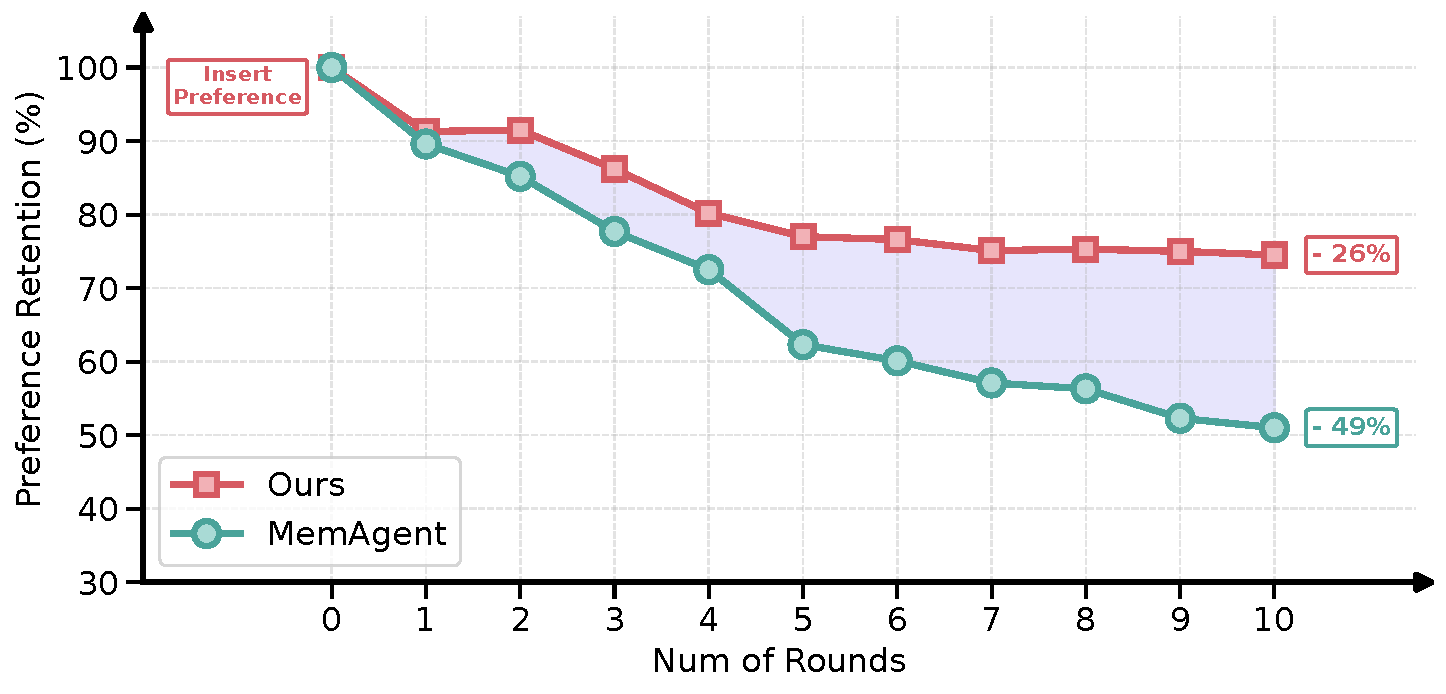
\includegraphics[width=0.89\linewidth]{img/preference_retention_gap.pdf}
\caption{Preference retention during multi-round memory evolution on PrefEval (Explicit). We insert a user preference at round 0 and then run memory evolution for subsequent rounds, where each round uses a 4K-token dialogue context. A strong judge model (\texttt{Gemini-2.5-Pro}) verifies whether the preference remains in the memory bank after each round.}
\label{fig:preference_retention_gap}
\end{figure*}
\begin{figure}[!htbp]
\centering
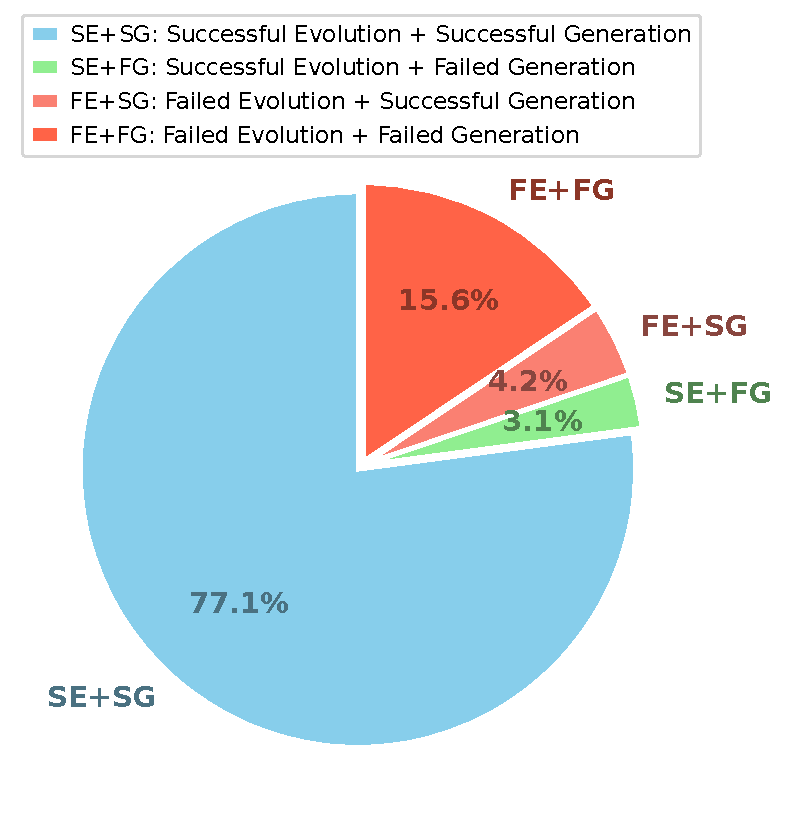
\includegraphics[width=0.89\linewidth]{img/pie-error-analysis.pdf}
\caption{Error analysis decomposing failures into the memory evolution stage and the response generation stage. We use the same setup as Figure~\ref{fig:preference_retention_gap}, where successful evolution means the memory bank captures the user preference, and successful generation means the final answer is correct given the evolved memory.}
\label{fig:error-analysis}
\end{figure}

Figure~\ref{fig:preference_retention_gap} directly tests whether our method can preserve useful user preference information inside the memory bank throughout multi-round memory evolution. We use PrefEval (Explicit) because the preference is inserted at the beginning (round 0), which makes retention measurable and avoids ambiguity about when the preference should appear. After inserting the preference, we run multi-round evolution with a fixed 4K-token context per round, and ask \texttt{Gemini-2.5-Pro} to judge whether the memory bank still contains the inserted preference. At round 0, both methods have 100\% retention by construction, after which their retention curves diverge rapidly as rounds increase: MemAgent exhibits a steep and nearly monotonic decay, dropping to roughly 51\% retention by round 10, whereas our method degrades much more slowly and remains around 74\% at round 10. This yields a substantially smaller absolute decrease in retention for our method (about 26\%) compared to MemAgent (about 49\%), and the growing shaded gap indicates that the advantage accumulates over time rather than being a one-off effect. 
Qualitatively, this behavior aligns with our design goal. Specifically, by introducing an induced memory-update guideline to regulate what to keep, refine, or delete, our evolution process is less prone to overwriting or dilution of the initially injected preference under long interaction histories.
In contrast, MemAgent appears more vulnerable to preference drift and forgetting as the number of rounds increases, since later interactions can introduce competing signals and noisy content that interfere with the original preference.

\begin{figure*}[!htbp]
\centering
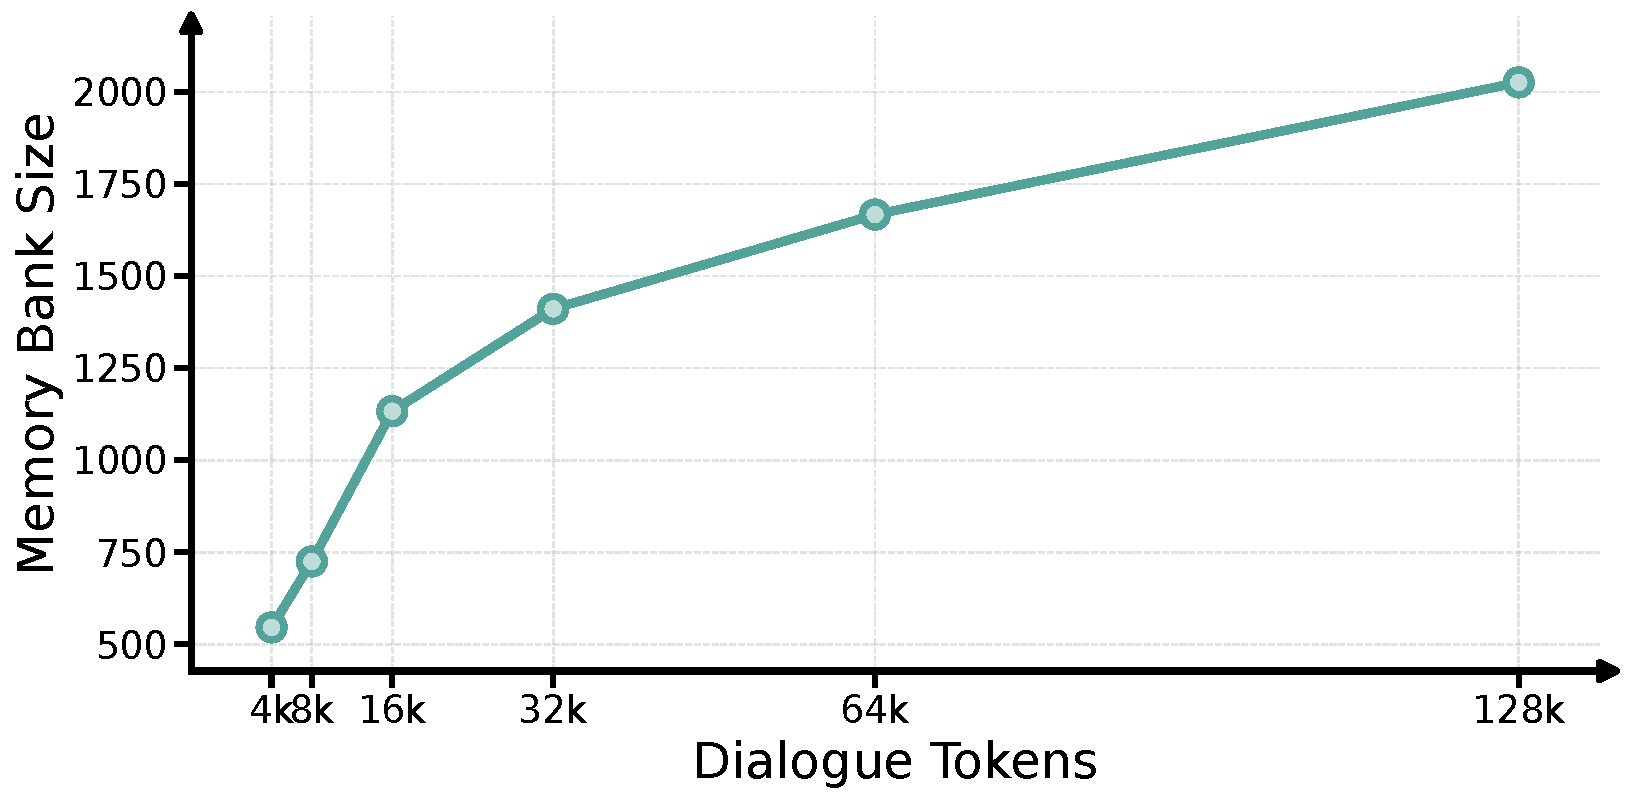
\includegraphics[width=0.48\linewidth]{img/memory_bank_size.pdf}
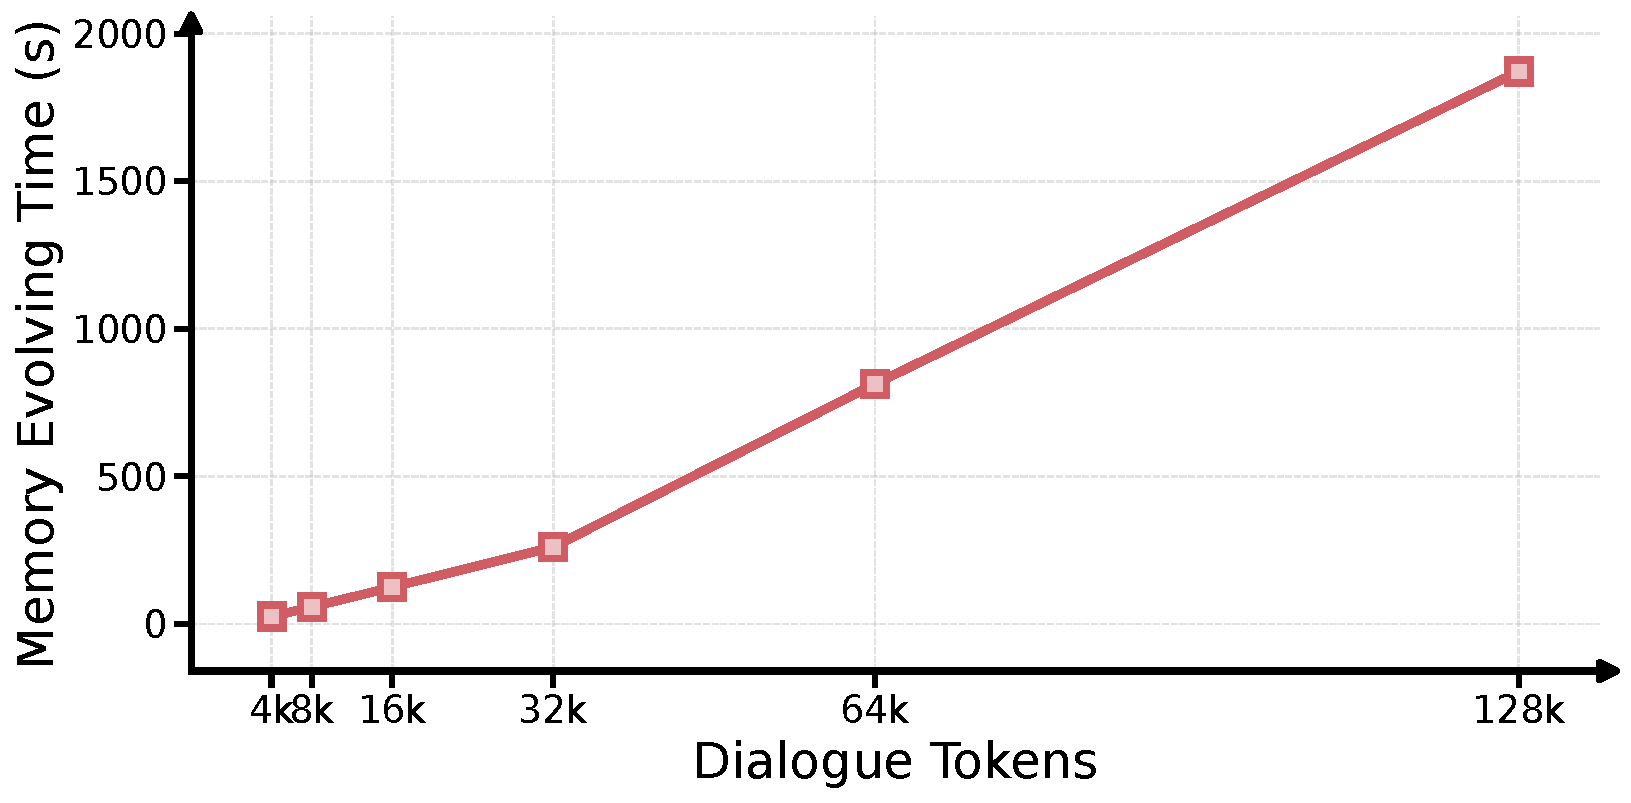
\includegraphics[width=0.48\linewidth]{img/memory_evolving_time.pdf}
\caption{Scaling analysis on PersonaMem (128K). We increase the total dialogue tokens (each evolution round processes 4K tokens) and report the resulting memory bank size (left) and memory evolving time (right).}
\label{fig:scaling}
\end{figure*}

\begin{figure*}[t]
    \centering

    \begin{subfigure}[t]{0.42\linewidth}
        \centering
        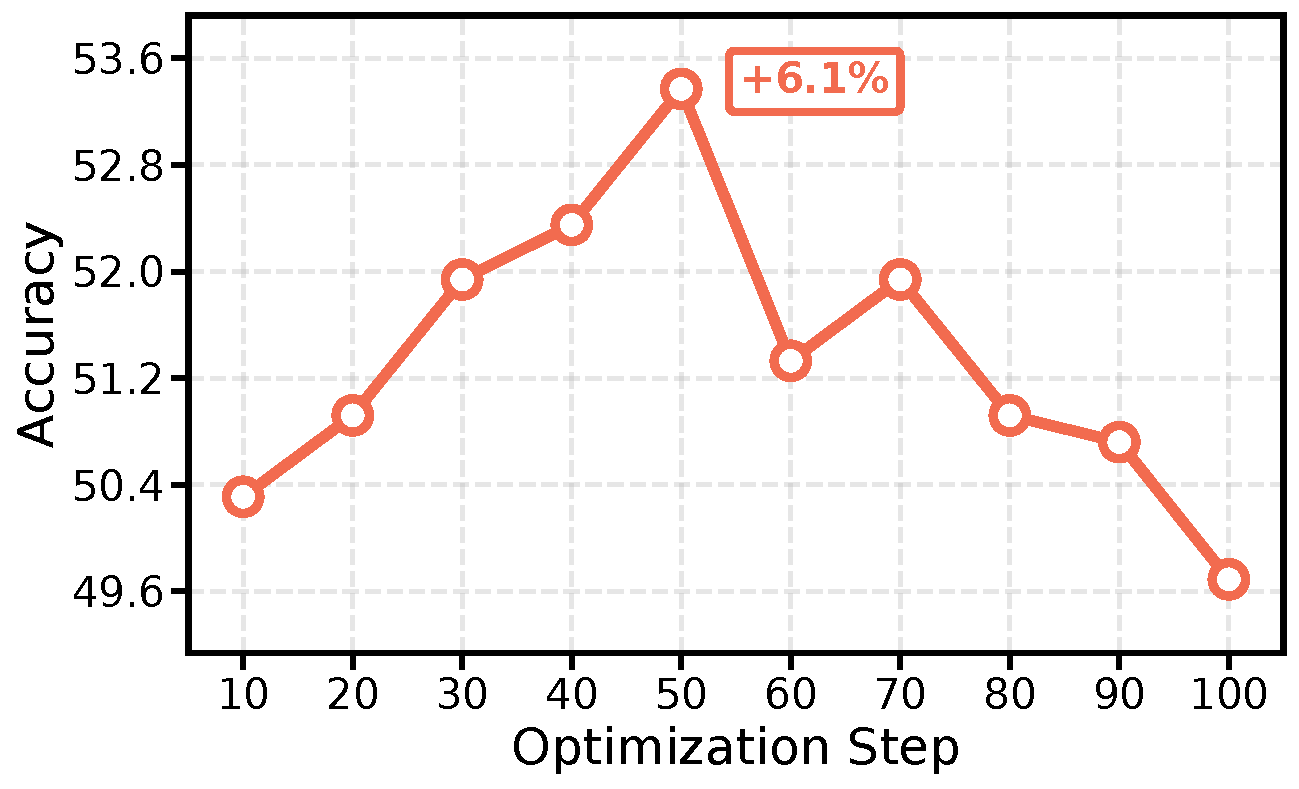
\includegraphics[width=\linewidth]{img/optim_step_personamem_32k.pdf}
        \caption{PersonaMem (32K)}
        \label{fig:optim-step-personamem-32k}
    \end{subfigure}
    \begin{subfigure}[t]{0.42\linewidth}
        \centering
        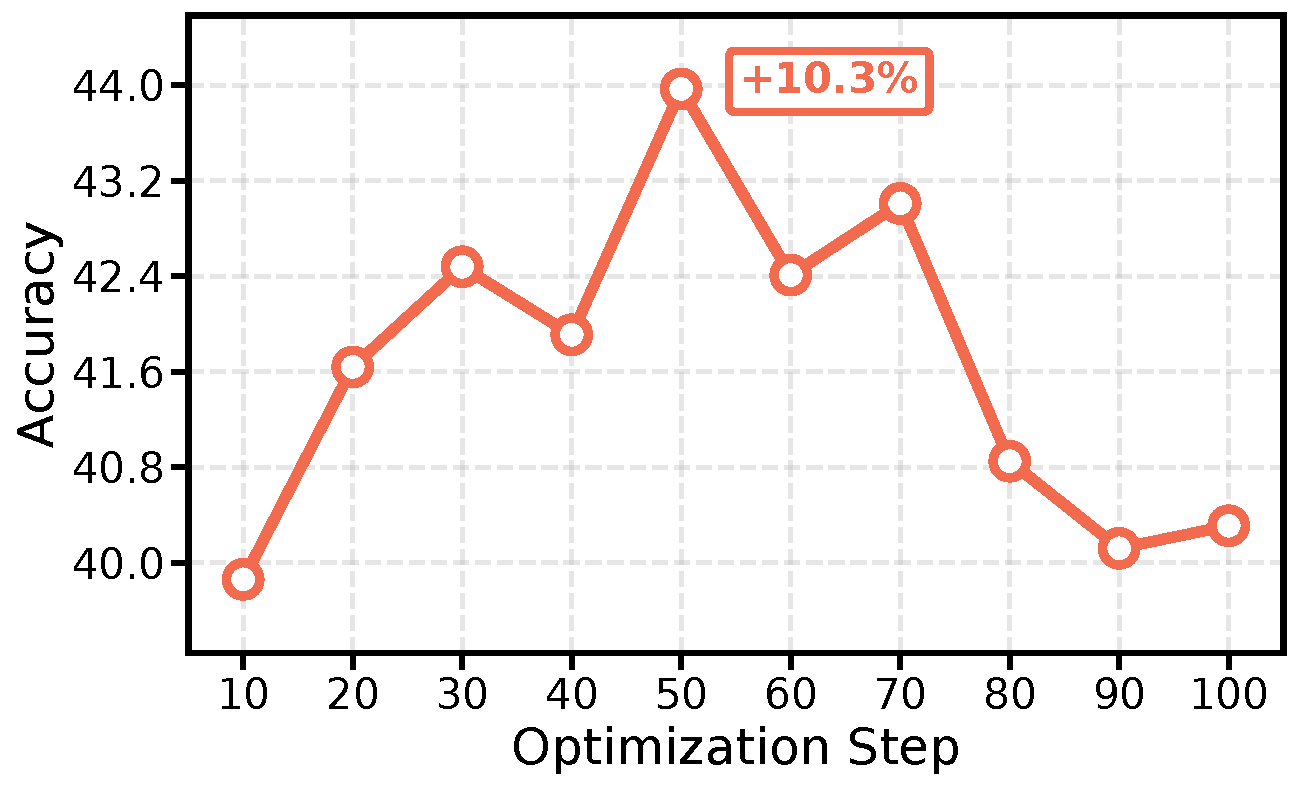
\includegraphics[width=\linewidth]{img/optim_step_personamem_128k.pdf}
        \caption{PersonaMem (128K)}
        \label{fig:optim-step-personamem-128k}
    \end{subfigure}

    \vspace{0.6em}

    \begin{subfigure}[t]{0.42\linewidth}
        \centering
        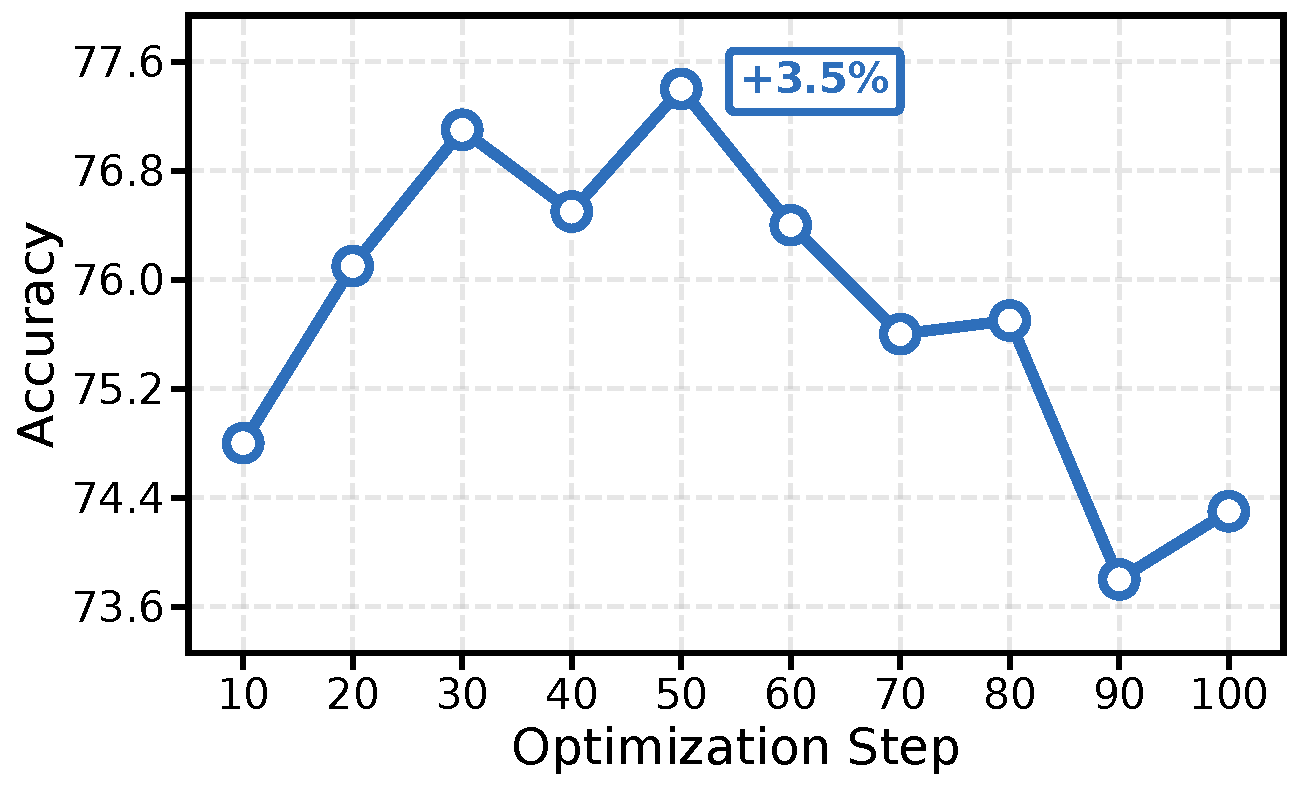
\includegraphics[width=\linewidth]{img/optim_step_prefeval_explicit.pdf}
        \caption{PrefEval (Explicit)}
        \label{fig:optim-step-prefeval-explicit}
    \end{subfigure}
    \begin{subfigure}[t]{0.42\linewidth}
        \centering
        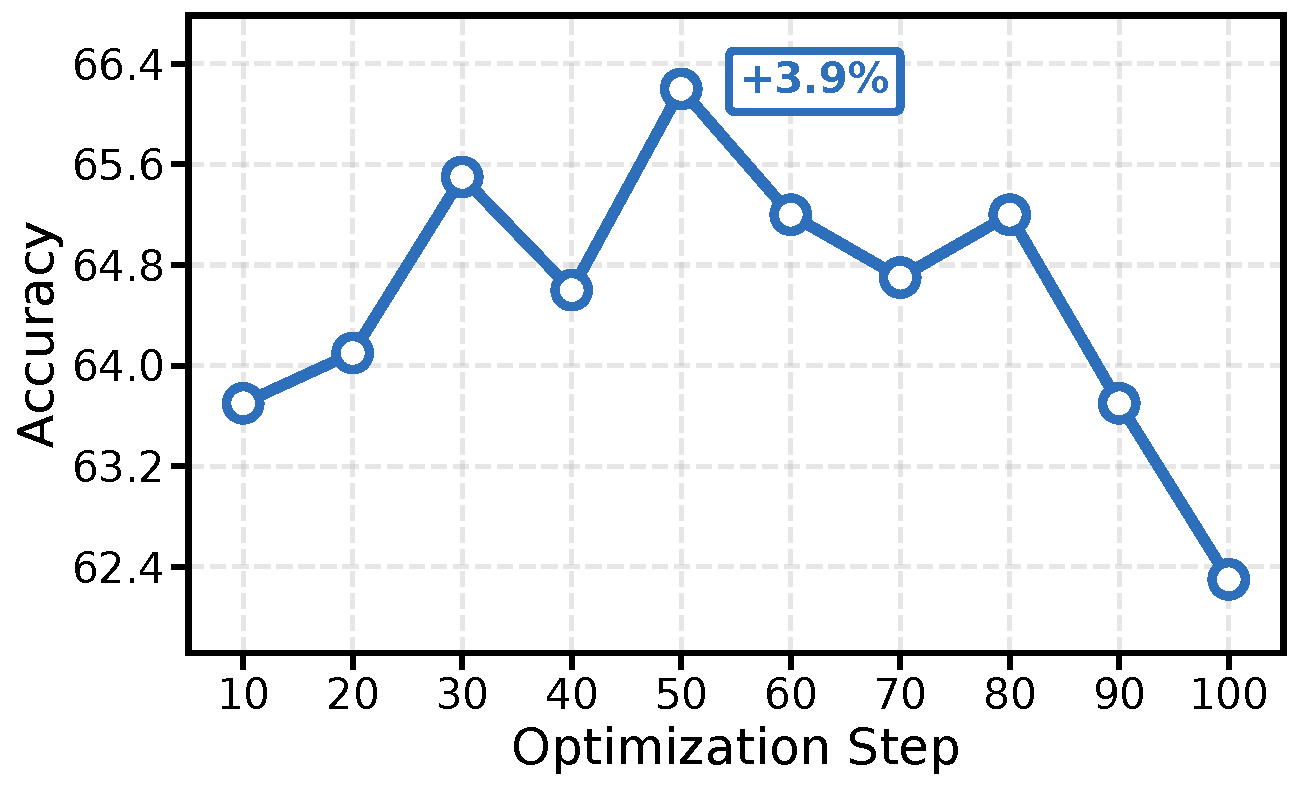
\includegraphics[width=\linewidth]{img/optim_step_prefeval_implicit.pdf}
        \caption{PrefEval (Implicit)}
        \label{fig:optim-step-prefeval-implicit}
    \end{subfigure}
    \caption{Hyperparameter analysis of optimization steps. The relative gains ($+\Delta\%$) are computed w.r.t.\ the performance at step 10.}
    \label{fig:optim-step-hparam}
\end{figure*}


\subsection{Error Analysis}
Figure~\ref{fig:error-analysis} breaks down errors according to whether they originate from the memory evolution stage or the response generation stage under the same preference-retention setup as Figure~\ref{fig:preference_retention_gap}. The dominant category is SE+SG (Successful Evolution + Successful Generation) at 77.1\%, indicating that in most cases the system both captures the user preference in the memory bank and leverages it to produce a correct response. The remaining 22.9\% errors are split across three failure modes: SE+FG accounts for 3.1\%, showing that even when the preference is correctly stored, generation can still fail to use it; FE+SG accounts for 4.2\%, suggesting that correct answers can occasionally be produced despite imperfect preference capture (e.g., the model may rely on residual context cues rather than the memory bank); and FE+FG accounts for 15.6\%, which is the largest failure category and highlights that missed or incorrect preference capture during memory evolution often cascades into downstream response failures. Overall, this decomposition suggests that improving the reliability of the evolve stage, i.e., making it more consistent in capturing and preserving preferences, should yield the largest payoff. The comparatively small SE+FG slice indicates that, although present, generation errors are not the primary bottleneck in this setting.


\subsection{Effect of Training Steps on RL-Based Baselines}

\begin{figure}[t]
    \centering
    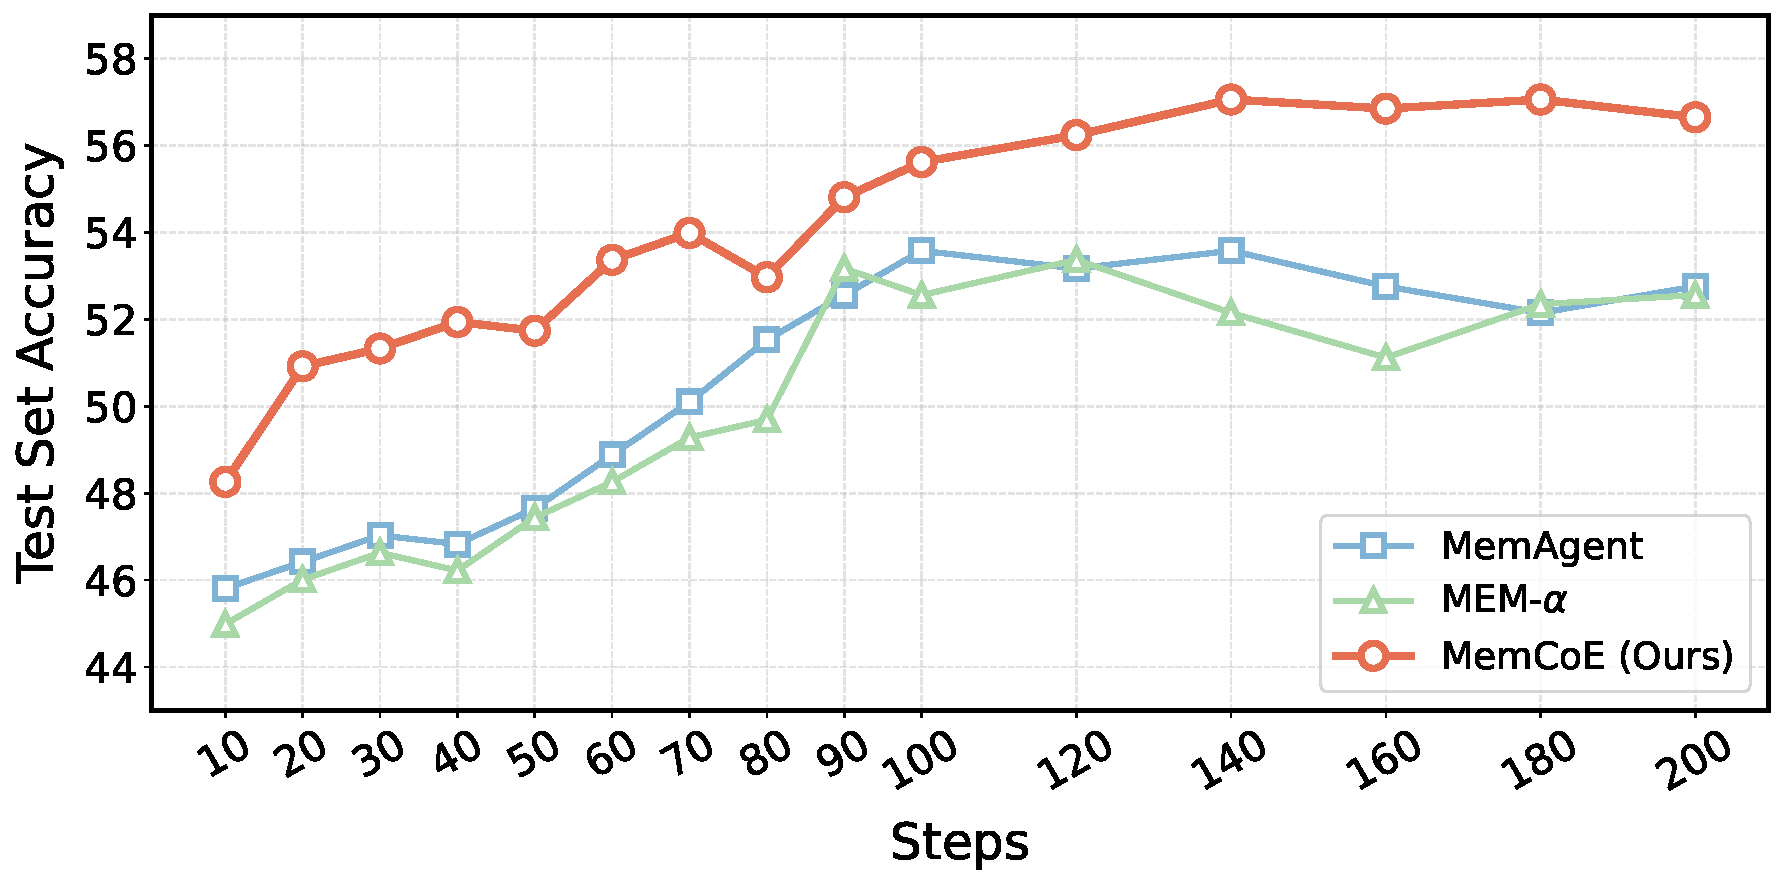
\includegraphics[width=1\linewidth]{img/training_curves.pdf}
    \caption{Test set Accuracy of RL-based baselines across RL training steps.}
    \label{fig:training_steps}
\end{figure}

To verify that the performance gap between MemCoE and RL-based baselines is not attributable to insufficient baseline training, we conduct a training-step study under an identical data budget and experimental setting: 300 sampled PersonaMem training examples, batch size 4, and evaluation on PersonaMem-32K, varying only the number of RL update steps up to 200. As shown in Figure~\ref{fig:training_steps}, both MemAgent and MEM-$\alpha$ reach a clear performance plateau around steps 100--140, with MemAgent peaking at 53.58 (steps 100/140) and MEM-$\alpha$ peaking at 53.37 (step 120), after which neither baseline exhibits consistent improvement—confirming that both models have converged within the given budget. Despite this, MemCoE continues to outperform the best checkpoints of both baselines by a substantial margin throughout training, demonstrating that the observed accuracy gap stems primarily from MemCoE's architectural design rather than any insufficiency in baseline training.


\subsection{Scaling Analysis}
Figure~\ref{fig:scaling} analyzes how our memory system scales with longer dialogue context on PersonaMem (128K) using 4K tokens per evolution round. As the dialogue tokens grow from 4K to 128K, the memory bank size increases from roughly 500 to around 2,000, and the curve is sublinear: it grows faster in the short-context regime and then gradually flattens as the history lengthens, which is consistent with consolidating stable information while removing redundant or outdated content to \textbf{keep memory overhead under control}. Meanwhile, the memory evolving time increases smoothly with dialogue length and follows an \textbf{approximately linear trend}, remaining well-behaved across the entire range; this indicates that the computational cost scales predictably with the amount of dialogue processed per round, with the slowly expanding memory bank introducing only a mild additional overhead in longer contexts.


\subsection{Optimization Step Analysis}
Figure~\ref{fig:optim-step-hparam} studies the number of optimization steps used in \moduleone for Memory Guideline Induction. Across all four settings, performance improves from the initial configuration and reaches a clear peak at an intermediate step budget, with the best results achieving relative gains of +6.1\% (PersonaMem 32K), +10.3\% (PersonaMem 128K), +3.5\% (PrefEval Explicit), and +3.9\% (PrefEval Implicit) compared to the 10-step setting. When the step count is too small, the guideline updates are likely under-developed: the aggregated textual gradients have limited opportunity to accumulate recurring error patterns across batches, so the induced guideline remains close to the initial prompt and cannot consistently regulate memory operations. Conversely, when the step count becomes large, the curves show a downward trend after the peak, suggesting diminishing returns and instability: repeated natural-language edits can over-specialize the guideline to feedback from later batches, or amplify small contradictions across textual gradients, which in turn weakens its ability to \textbf{generalize across histories and query types}. Overall, the results indicate that \moduleone benefits from enough iterations to consolidate batch-level critiques into a robust global policy, but requires a moderate step budget to avoid drifting away from broadly useful memory-update principles.


\subsection{Comparison with TextGrad}
\label{subsec:prompt_opt}

To further validate MGI, we compare against TextGrad~\cite{yuksekgonul2025optimizing}, a strong general-purpose prompt optimizer, under the PersonaMem (32K) setting. Results are shown in Table~\ref{tab:prompt_opt}: TextGrad improves over the manual prompt but still lags behind MGI by a substantial margin. This gap highlights that general prompt optimization is insufficient for our memory-evolution setting, where updates must be grounded in long-horizon trajectories. The results support that MGI's trajectory-grounded contrastive signal and batch aggregation are critical for inducing a high-quality memory guideline.

\begin{table}[h]
\centering
\caption{Comparison with prompt optimization methods on PersonaMem (32K). $^*$ indicates statistically significant improvement over the second-best baseline (two-sided $t$-test, $p < 0.05$).}
\label{tab:prompt_opt}
\begin{tabular}{lc}
\toprule
\textbf{Method} & \textbf{PersonaMem (32K)} \\
\midrule
Manual Prompt         & 48.25 {\scriptsize $\pm$ 0.68} \\
TextGrad & 49.83 {\scriptsize $\pm$ 0.83} \\
MemCoE (w/ only MGI)  & \textbf{53.28} {\scriptsize $\pm$ 0.76}$^*$ \\
\bottomrule
\end{tabular}
\end{table}

